Consider the following feedback system, with the Bode plot for $G(s)$ shown on the right. $G(s)$ has one pole in the right half plane (unstable pole).\\
\begin{minipage}{2.5in}
\begin{center}
\resizebox{2.5in}{!}{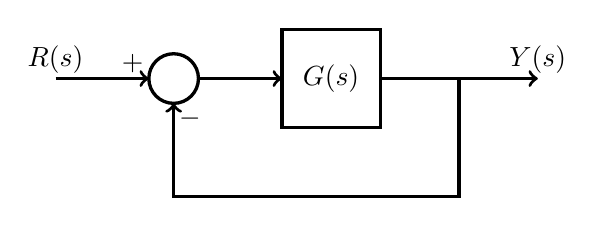
\begin{tikzpicture}[scale=1,inner sep=0pt,outer sep=0pt,very thick,
sysblock/.style={draw,rectangle,inner sep=2pt,minimum width=1.25cm,minimum height=1.25cm,very thick}]
\draw (2,0) node[draw,circle] (sum1) {$\rule{0pt}{18pt}$};
\draw (4,0) node[sysblock] (G) {$G(s)$};
\draw[->] (.5,0) node[above=2pt] {$R(s)$} -- (sum1.180) node[above left=2pt] {$+$};
\draw[->] (sum1.0)  -- (G);
\draw[->] (G.0) -- ++(2,0) node[above=2pt] {$Y(s)$};
\draw[->] (G.0) ++(1,0) -- ++(0,-1.5) -| (sum1.-90) node[below right=2pt] {$-$};
\end{tikzpicture}}
\end{center}
\end{minipage}
\begin{minipage}{4.5in}
\includegraphics[width=5in]{\mainfolder/LectureNotes/\lecturefolder/HomeworkProblems/Problem10/bode}
\end{minipage}
\begin{enumerate}
\item Sketch the Nyquist plot. Mark on the Bode plot the magnitude and phase when the Nyquist plot crosses the real or imaginary axis.
\item Determine if the feedback system is stable in closed loop.
\end{enumerate}